\documentclass{vldb}
\usepackage{graphicx}
\usepackage{balance}
\usepackage{algorithm2e}
\usepackage{tabularx}
\usepackage{placeins}


\begin{document}

% ****************** TITLE ****************************************

\title{MemDB: A Fast, Scalable In-Memory Storage Engine For NoSQL Secondary Indexes}


% ****************** AUTHORS **************************************

\numberofauthors{1}
\author{
\alignauthor
Sarath Lakshman\\
       \affaddr{Couchbase, Inc.}\\
       \email{sarath@couchbase.com}
}

\maketitle

\begin{abstract}
MemDB is a fast indexing storage engine designed for NoSQL database systems. MemDB keeps all data in memory. The architecture is crafted towards scalability, efficiency and performance for asynchronously updated secondary indexes. The MemDB engine is capable of scaling well with modern multicore systems and throughput scales almost linearly with the number of available CPUs. Even though all data is stored in DRAM, we also offer ability to take full database snapshot, fast load and rebuild from disk snapshots. The core data storage leverages lock-free data structures to avoid contentions in data read-write access. The storage engine offers point-in-time snapshots of the index for highly consistent query results. Modern OLTP application workloads require low latency and high throughput access to the data. Couchbase high performance document database stores billions of documents distributed over many nodes on disk+memory. Secondary indexes are usually defined on simple fields having few bytes in length. This makes in-memory indexes a viable option for scale out databases for offering fast indexes.
    We have integrated MemDB into the Couchbase global secondary indexes (GSI) and observed an order of magnitude improvement in performance compared to disk based storage engine. With GSI system running on a 32-core machine, we observed an index build throughput of 200k/s and index update throughput of 175k/s. The raw MemDB throughput observed for similar workload was 600k/s and 500k/s respectively. The engine was able to saturate all 32-cores for its operation. We have benchmarked MemDB up to 144-cores system and verified that we do not have any bottlenecks in scaling.
\end{abstract}




\section{Introduction}
The nature of data is distributed and indexes are centralized in nature. The analogy of a library of books clearly states an example. Different books are stacked in a distributed manner, but the indexes for books are placed in one or two racks and they are small in nature. It is always better to have smaller number of fat index nodes since it reduces the need for scatter gather and delivers lower latency. Hence, single indexer node performance matters. Smaller number of servers also helps in reducing costs and avoids load imbalances caused by partitioning. This paper presents MemDB, a high performance storage engine designed for secondary indexing.

    There are a number of advances in the field of high performance KV storage engines recently. ForestDB, LevelDB, RocksDB, WiredTiger, etc are the mainstream ones in the ecosystem. While they solve the problem of primary storage nicely for different use cases, they are not good enough for asynchronously updated secondary indexes. They require further specializations in the storage engine to tap be maximum efficiency and performance. While the primary data storage system solves the challenge of storing large volumes of data with each documents of large in size (Typically 10KB to 512KB), secondary indexes solve the problem of storing large number of small keys (Typically 25B to 512B) and offer low latency. In most use cases indexes can completely fit in the DRAM. MemDB offers a fully DRAM resident high performance storage system for indexes. Most KV storage systems focuses few cores scalability and are unable to deliver performance scalability with increasing number of cores. Scaling single index performance by increasing number of cores is attractive.
    
    The backbone of MemDB is a lock-free skiplist and an MVCC system to offer point in time snapshots. The lock-free nature of the data structure is key to scalability with number of cores. We also avoid any duplication of data in memory across data structures and also avoid unnecessary cross data structure accesses within the indexing storage system. This is impossible to achieve using a general purpose KV storage engine for indexes. MemDB supports multiple writers to make use of all the CPUs available in the system. System can hold multiple snapshots in memory with bare minimal overhead and snapshots are immediately garbage collected when the users of the older snapshots go away. Each writer can operate independently without lock-based coordination. It also offers fast snapshotting facility to create point-in-time snapshots. The time taken for creating snapshots has very significant effect on indexing update performance. Usually storage engine buffers all writes into a write ahead log (WAL) and apply them all together into main data structure atomically when a commit is invoked to create a new snapshot. But, commit is time consuming since it has to read back all the entries from the WAL and apply them and make structural modification to the main data structure. The time taken by the commit causes head of line blocking for the indexing update pipeline and causes delays and degrades index update performance. Secondary indexing system typically creates around 100 snapshots every second. While all data is kept in the memory, MemDB also offers to backup full index snapshots to disk periodically. Disk snapshotting makes use of multi CPU parallelism for data structure scan and maximizes disk utilization with sequential IO of large block sizes. Recovery is also very fast since it builds the data structures in bottom-up fashion and makes use of all available CPUs. MemDB also writes only the bare secondary keys to the disk for each snapshot. Storage is not wasted because of write-amplication unlike general-purpose KV storage engines.


\section{Background}
Secondary indexing performance is a key factor for the success of any database system.  The traditional disk based database systems provide secondary indexes, which are updated synchronously with the primary index. If you have a number of secondary indexes, it has to pay the cost of updating all secondary indexes during the primary index update and eventually this becomes a scalability bottleneck. If you want to experience seamless scaling, we should be able to scale primary indexes and secondary indexes independently. Couchbase 4.0 introduced multidimensional scaling (MDS) to scale different set of services independently. Couchbase is a distributed document database with JSON at its heart. In the context of JSON documents, secondary indexes are defined on a field in the document. JSON documents are stored in the Couchbase with an identifier (maximum of 256 bytes). Couchbase offers bucket namespaces for grouping your documents. Asynchronous indexing poses several challenges in index maintenance. Nodes with index role host indexes and indexer process receives new versions of the documents through Database Change Protocol (DCP). The documents are sent in de-duplicated small batches called snapshots. Even though the document versions are sent through the DCP in the order they have been received from the applications, within a DCP snapshot, order is irrelevant since they preserve only the latest version for each document in a snapshot. This is an optimization to save network bandwidth and disk bandwidth for consumers of DCP. However, this introduces an additional responsibility at the consumers. For data received to be consistent with respect to the main document storage, the consumer should always apply all the documents from a snapshot atomically. Any partial application of documents from a snapshot results in inconsistency.

    The main task of index storage engine is to receive document versions in DCP snapshot batches and apply corresponding changes to the index, snapshot by snapshot. Each document version received consists of a document-id and value of interested secondary JSON field. Secondary index supports full tables scan, range scan, lookup queries and count range queries. GSI indexing engine has two types of index update schemes: Initial build and Incremental update. Suppose that an index is build by using existing documents in the bucket, it is called initial build. Any further update to the index to keep up with the changes happening to the indexed documents is called incremental update.


\section{Storage Engine Operations}
Let us walk through some examples for secondary indexing on JSON documents. A document, employee-01 has a JSON body {“id”: 1022, “city”: “Bangalore”, “title”: “Software Engineer”}. If we create a secondary index on “city”, we should be able to query against the index based on city. For the above document, index should have an entry [“Bangalore”, “employee-01”]. Now let us say that the employee changed his city to “MountainView”. The index should now reflect the change and the entry should become [“MountainView”, “employee-01”]. Here comes the problem. From the index how do we delete the previous entry before updating with the new one ?

    Under the cover, storage engine maintains two data structures for index maintenance.  One for keeping the mapping from document-id to current-secondary-value and other for storing secondary values alone. The first one is called backstore and the latter is called mainstore. So, in the above example when a new document version {“id”: 1022, “city”: “MountainView”, “title”: “Software Engineer”} arrives, first we will retrieve the previous secondary value for employee-01 from backstore. Then that secondary entry would be removed from mainstore before new entry is added to the mainstore.
    

  Storage engine performs the following sequence of operations:
  
\begin{algorithm}
\SetAlgoLined
\KwData{docid, secKey}
 \BlankLine
prevSecKey= backstore.Lookup(docid)\;

  \If{prevSecKey}{
   backstore.Delete(docid)\;
   mainstore.Delete([prevsecKey, docid])\;
   }
   
   backstore.Insert(docid, secKey)\;
   mainstore.Insert([secKey, docid])\;
 \BlankLine
 \caption{Secondary key insert/update operation}
\end{algorithm}

During initial index build, backstore.Lookup(docid) would always return nil since the documents are getting indexed for the first time. Initial build requires two operations less than the incremental update and hence initial build is faster than incremental update.

\section{Design}
MemDB system makes use of two data structures for storage. A lock-free skiplist for mainstore and a hash-table for backstore. The choice of skiplist for the main index storage is due its simplicity and high performance. It provides logarithmic access to the items in the store, while it provides linear time access within a key range.  The storage engine supports the following operations:

\begin{enumerate}
  \item Put
  \item Get
  \item Delete
  \item SnapshotIteration
  \item CreateSnapshot
  \item SaveToDisk
  \item RestoreFromDisk
\end{enumerate}

\begin{figure}
\centering
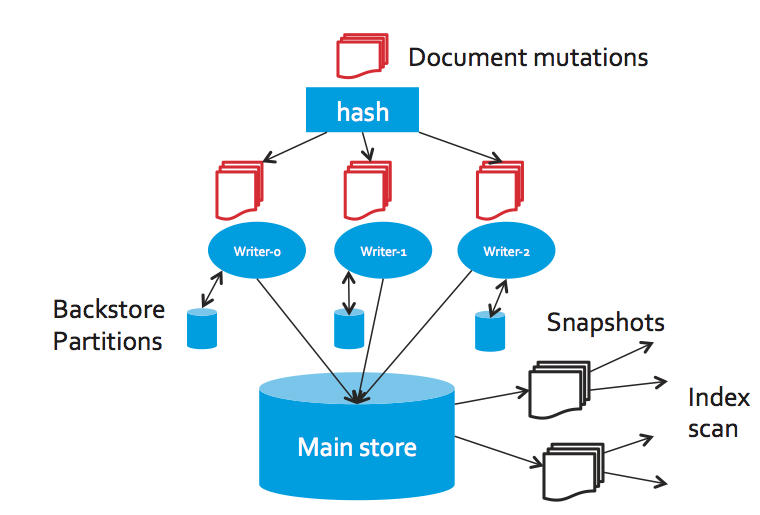
\includegraphics[scale=0.3]{images/fig-1}
\caption{Components in MemDB storage engine}
\label{fig:engine}
\end{figure}

MemDB supports multiple writers to make use of all the CPUs in the system. Indexer creates a number of writers equal to the number of CPUs and distributes the work among the writers. The distribution is based on hash of document-id. This will make sure that all secondary key mutations happening to the same document will always arrive in sequential order through the same writer and avoids any possibility for out of order mutations for a document. The purpose of backstore is to provide previous secondary key value for a document. It is a key lookup table and hence do not need to support any range lookups. The hash partitioning of documents by document-id also enables us to partition backstore per writer. Hence, backstore does not need to pay the cost of lockfree data structures for concurrent access. The backstore is only accessed for operations within a writer. Indexer generates mutation batches based on DCP snapshot boundary sequence numbers every 10ms for all the vbuckets. Indexer inserts all the mutations in the batch using all the writers and creates a MemDB snapshot. This snapshot is used by index queries for range scans. New snapshots are created every 10ms and older ones are garbage collected once they are unreferenced by all the queries. Let us look at the core components of the system.


\subsection{Lockfree skiplist}

\begin{figure}[h]
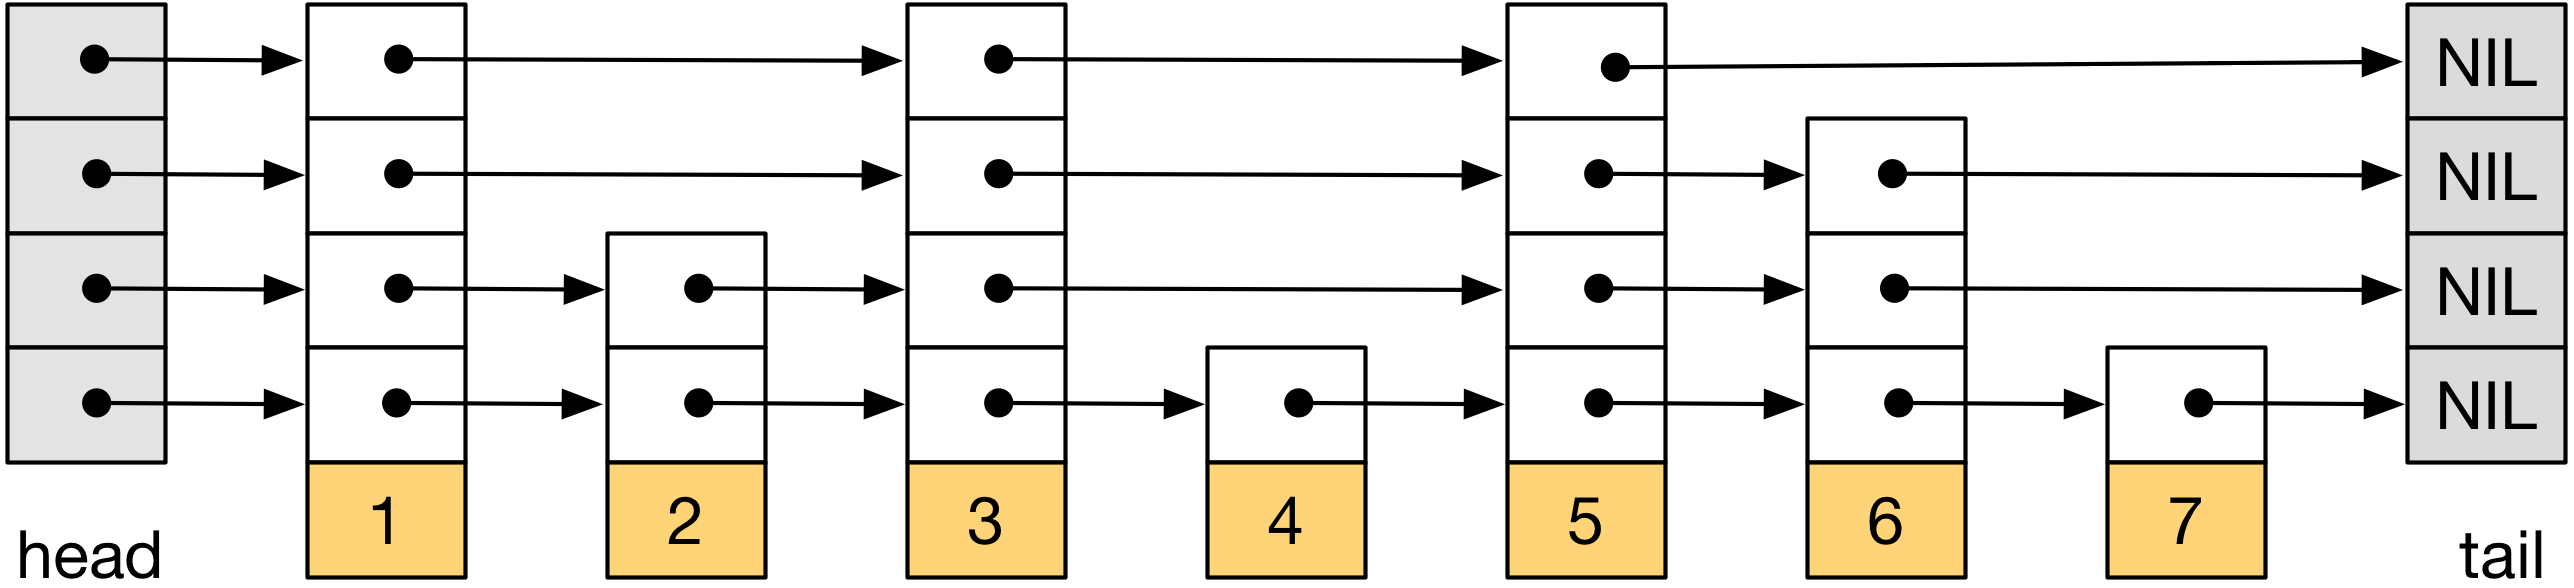
\includegraphics[scale=0.5]{images/fig-2}
\caption{Skiplist}
\label{fig:skiplist}
\end{figure}
Skiplist\cite{maurice:art-of-multproc} is a probabilistic balanced ordered search data structure. In simple words, we could describe it as a group of linked lists arranged in levels to facilitate binary search. The lowest level (level-0) is a singly linked list with n nodes. Each of the next higher level has 1/f nodes of the previous level. f is a configurable number that provides memory vs cpu tradeoff for the skiplist. Each node in the skiplist belongs to a level and it has next pointers equal to its level. The level of a node is decided probabilistically. Theoretically, skiplists consume only 1.33 next pointers per node. Measured statistics from our implementation also meets this expectation. In order to lookup or insert an item into the skiplist, it creates a path buffer table of previous and next node pointers in each level. Basically, it starts from the topmost level head node. Looks at the right node in the current level if it has greater value than the lookup value. If it is greater, it decrements its current level by one and compares the value with right node in the next level. If the value of the right node is equal or less, it sets current node as right node. It keeps on doing this until it reaches the level0 and finds a right node that is greater than the lookup value. 


The lockfree skiplist\cite{pugh:skiplist} uses the same algorithm but ensures that operations are serialized using CompareAndSwap (CAS) atomic primitives. All next pointer updates are done using CAS. If the CAS fails, it has to restart the operation by recomposing the path buffers. The lockfree implementation ideas come from lockfree linked list algorithm\cite{valois:lockfree-list}. The insertion into skiplist is straightforward using CAS. But the delete is tricky. In the above diagram, what happens if an insert is happening between node-2 and node-3 while node-2 is being deleted. It could lead to a condition where node-x got inserted successfully between node-2 and node-3 and node-2 could also be successfully deleted. It can cause missing inserts. This problem can also be solved using two-step delete operation.
 We need double CAS that takes a (isdeleted, pointer) for swap. If a node is deleted, deleted flag is marked.  In that case, insert will fail during CAS since it expected \textit{isdeleted} to be false. DCAS is not available on generic platforms and hence we simulated a DCAS using tagged pointers.
 
 \begin{figure}[h]
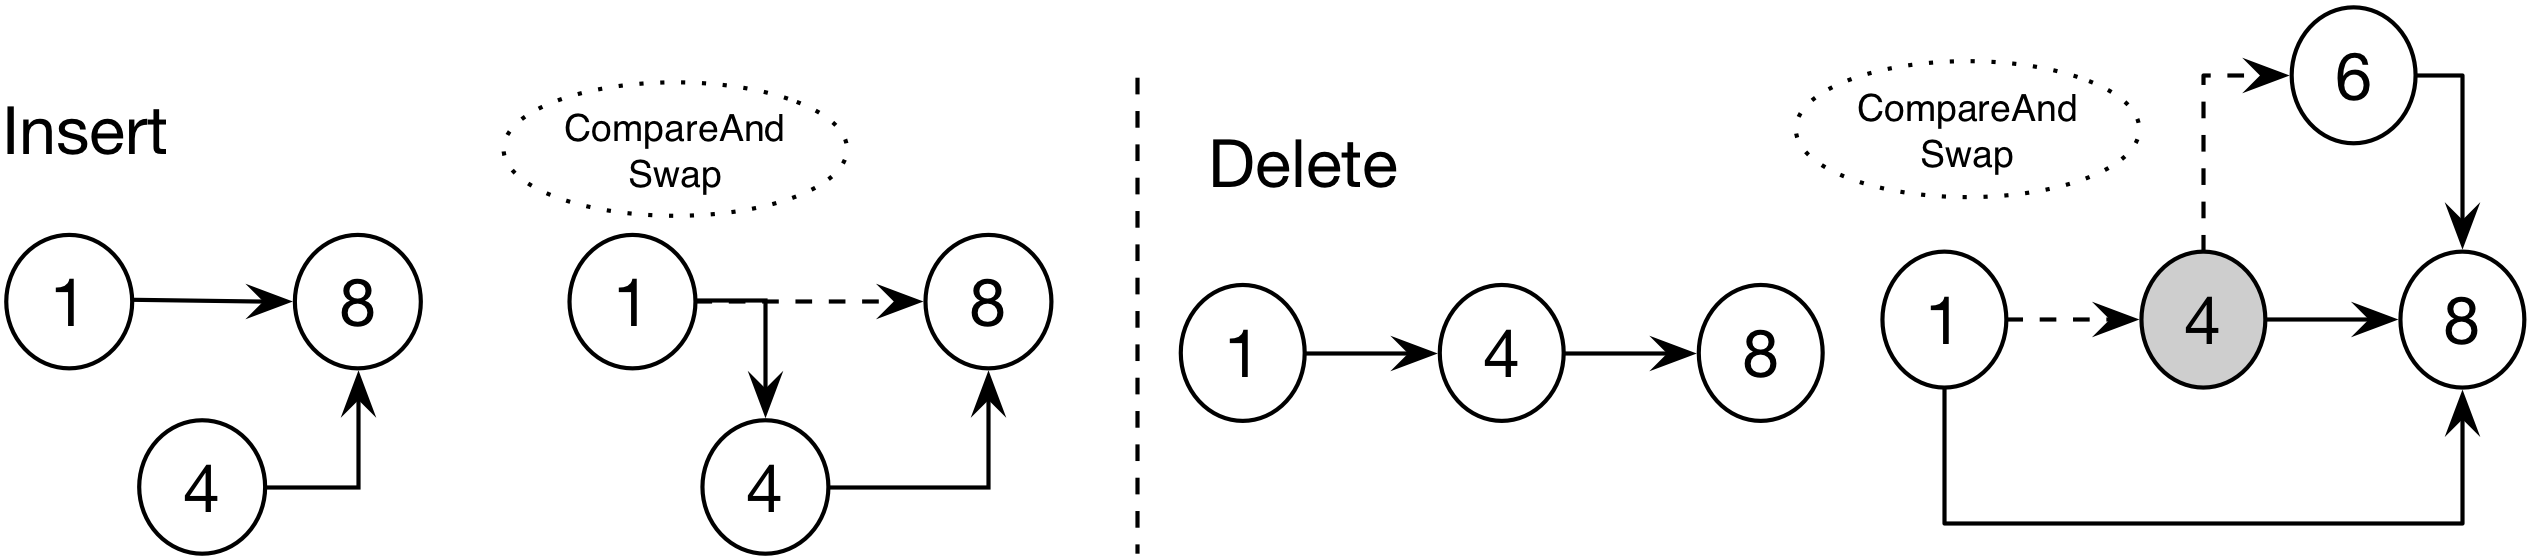
\includegraphics[scale=0.28]{images/fig-3}
\caption{Lockfree list insert/delete operations}
\label{fig:lockfree-list}
\end{figure}

\subsection{NodeTable}
The backstore is implemented using a hash table that maps document-id to skiplist node in the mainstore. The indirection from document-id to skiplist node avoids the need for a log(n) lookup in the mainstore to obtain the previous value of the secondary key. Also it avoids a log(n) lookup for deleting a node from the mainstore. The node table implementation avoids duplication of document-id and secondary key for mainstore and backstore.
    The node table consists of two hash tables. The first hash table is a fast-table which maps crc32hash(document-id) to pointer to the node in mainstore. But, the crc32 hash can lead to hash table collisions. To resolve collisions, we have a second hash table called slow-table. The slow-table maps crc32hash to a list of pointers to the mainstore nodes. The pointers are 64bit in size. One bit in the pointer value of fast-table is used to indicate whether collisions exist for the hash. This two-table approach is specific to improve the performance of golang implementation. Since fast-table has only fixed size types as key and value for the map, Golang garbage collection will not have to spend time in scanning the fast-table. Moreover, the node table is partitioned among MemDB writers, which further reduces the possibility for collisions. Hence, the number of entries in the slow-table should be very small. In an experiment of 100M items, we observed that 98M items stay in fast-table.
    During a document-id lookup in the node table, the document-id is hashed and corresponding candidate node pointers are retrieved. Now, for each skiplist node, we obtain the item and extracts document id for equality comparison to retrieve the exact node. We observed that node table is high performing and it can do 2M inserts/s, 4M gets/s and 3.5M updates/s with a single core.
    The high performance of backstore is desirable in handling key delete broadcast across all indexer nodes for range-partitioned indexes. 

\subsection{MVCC Layer}
The MVCC system is the crux of the MemDB’s transactional snapshots. Snapshotting capability provides versioning of the database state point-in-time and ability to read from the snapshots by isolating any further changes that happens to the database. Multiple snapshots can co-exist at any point in time. In the secondary indexing context, we need to be able to apply a batch of operations atomically to the database and create consistent checkpoints in the database. Any query can be serviced only from these consistent checkpoints.

 \begin{figure}[h]
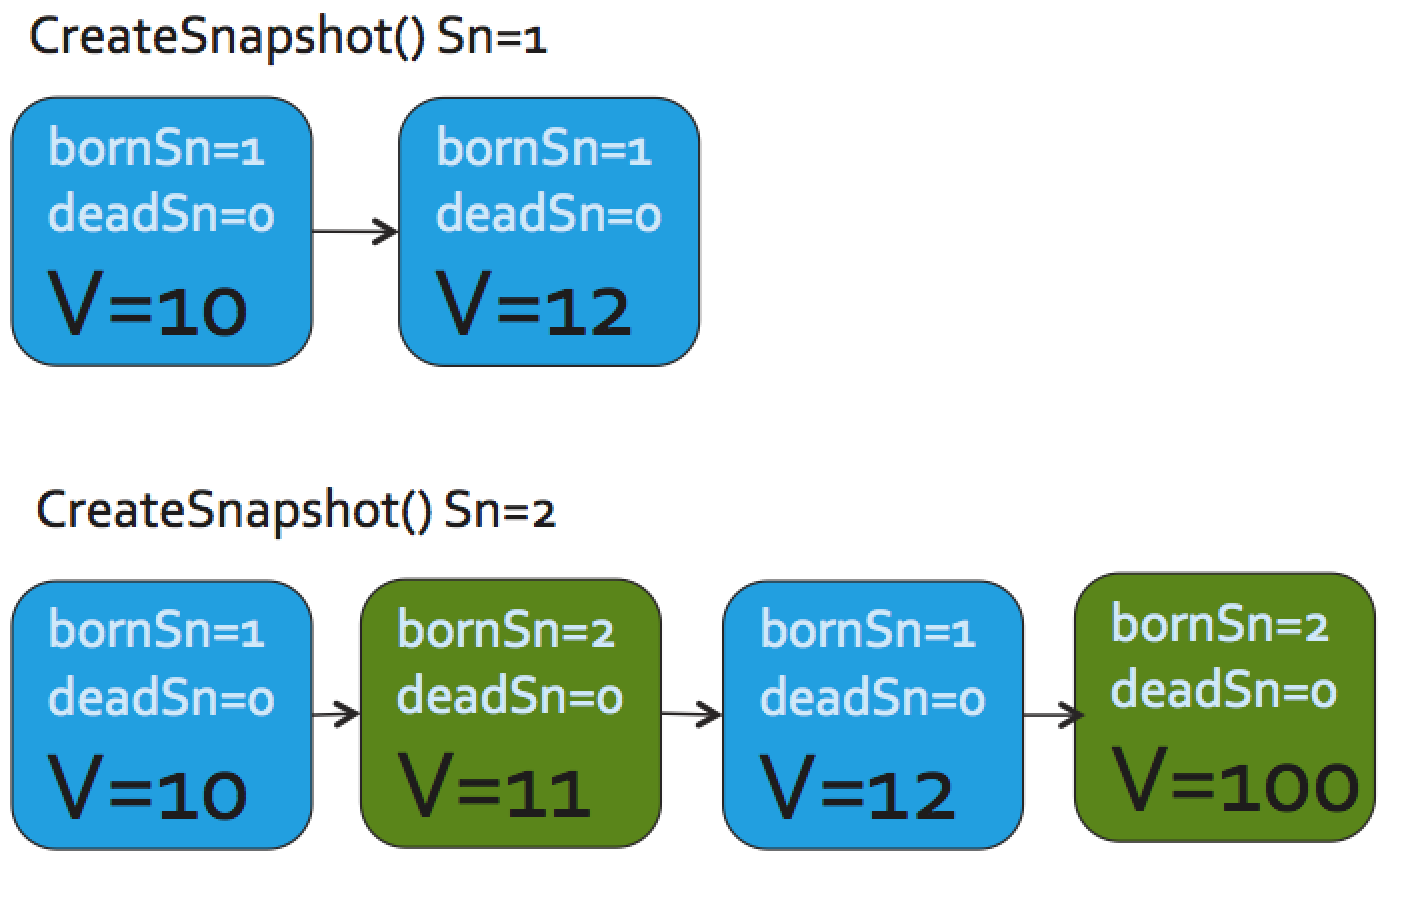
\includegraphics[scale=0.35]{images/fig-4}
\caption{Snapshotting based on versions of items}
\label{fig:mvcc}
\end{figure}

    MemDB system maintains a current snapshot session number which denotes the current active snapshot. Each item in the skiplist has two mandatory fields bornSn and deadSn. When a new item is inserted into the skiplist, bornSn is set to the current active snapshot number. bornSn provides the information of when this item was created. When an item is deleted from the skiplist, the corresponding node is located and its deadSn is set to the current active snapshot number. Physical removal from the skiplist is not performed immediately, but delayed and lazily performed during garbage collection. From bornSn and deadSn we can clearly state the lifetime of an item in the skiplist. Once an item is stamped with a bornSn, it is part of that immutable snapshot. When the application invokes CreateSnapshot() API, the global snapshot number gets incremented. Hence, snapshotting is a very cheap operation. All the items belonging to different snapshot sessions co-exist in the same skiplist ordered by (key, snapshot\_num).
    
\subsubsection{Snapshot Iterator}
The snapshot iterator is aware of the bornSn and deadSn metadata of the skiplist nodes. Snapshot iterator is associated with a snapshot object and upon creation of a snapshot iterator; the snapshot object reference count is incremented. The snapshot object holds a snapshot number.
 \begin{figure}[h]
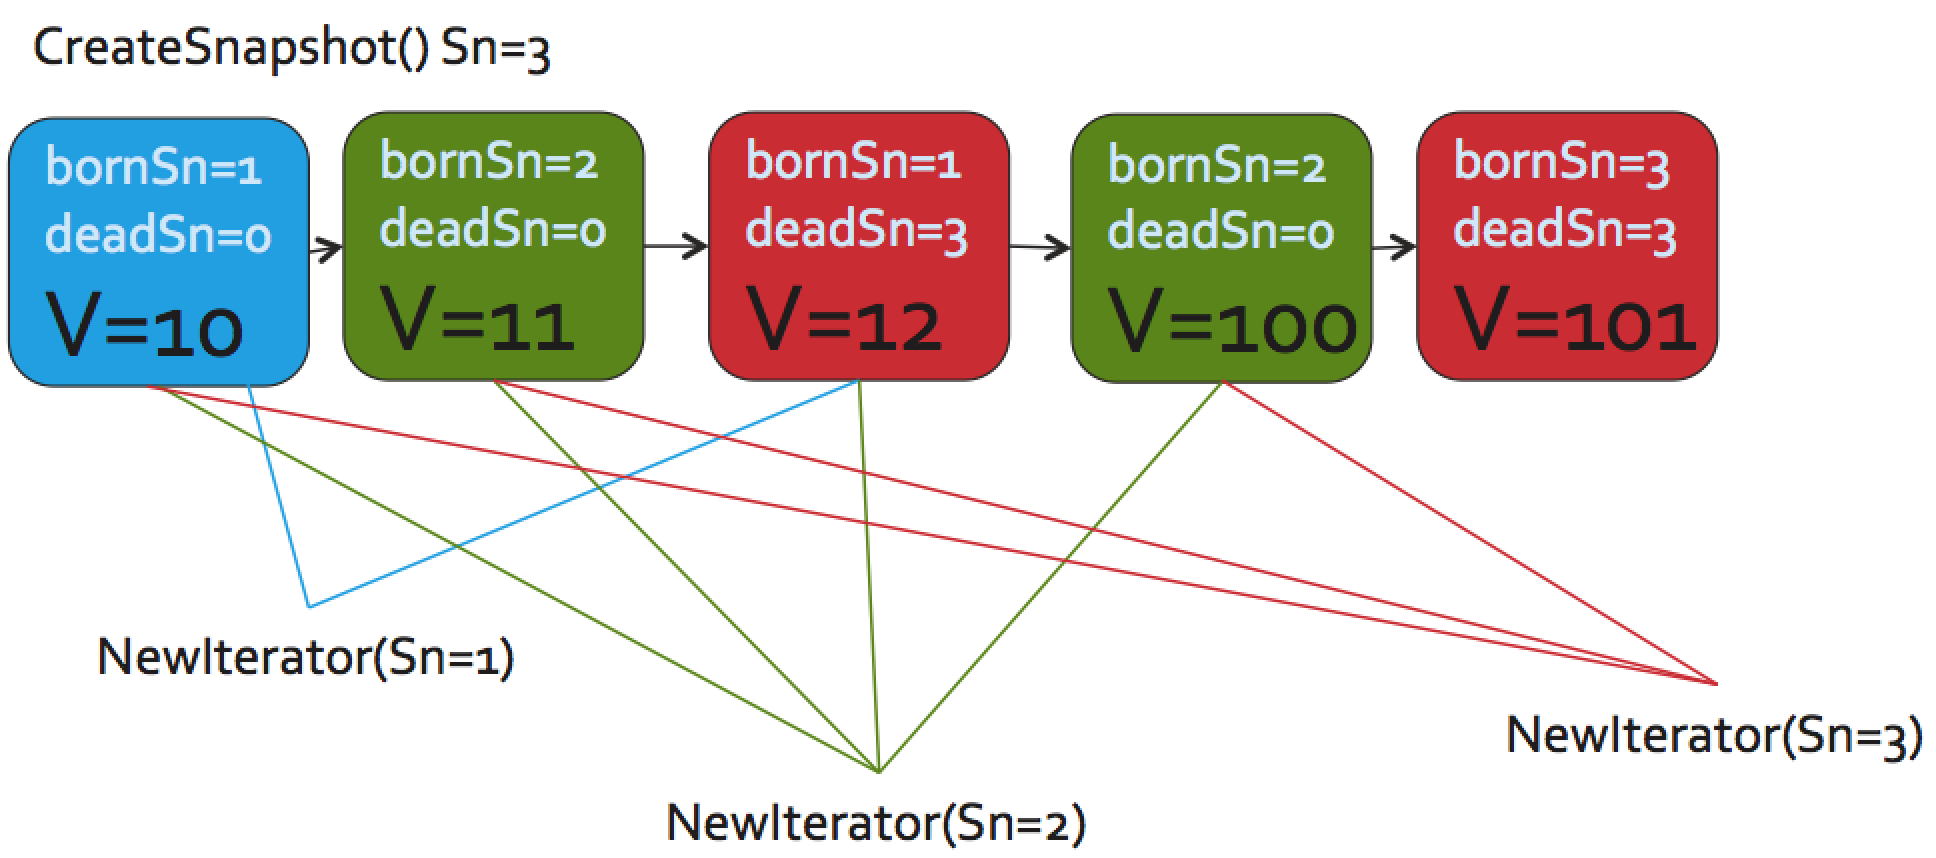
\includegraphics[scale=0.28]{images/fig-5}
\caption{Iterator operation on snapshot}
\label{fig:snap-iterator}
\end{figure}

The snapshot iterator uses bornSn and deadSn information to skip uninterested items during a range scan. If the iterator snapshot number is N, it will ignore all the items with bornSn > N and ignore all the items with deadSn <= N. In the above diagram, iterator with Sn=1 will only observe v=10 and v=12, while iterator with Sn=3 will observe v=11 and v=100.
    The key advantage of this system is that it allocates memory exactly equal to the number of items inserted in a snapshot. 

 \begin{figure}[h]
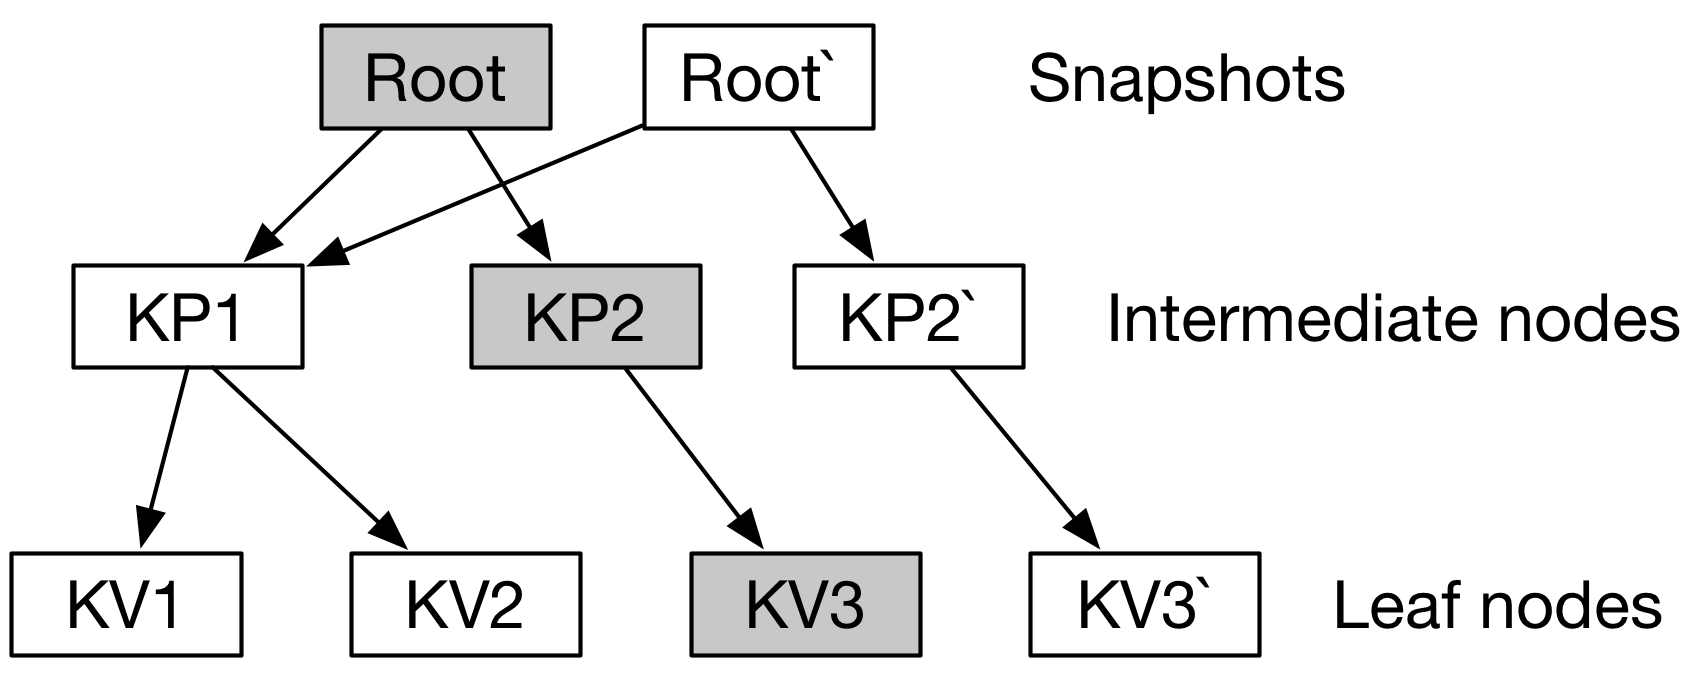
\includegraphics[scale=0.28]{images/fig-6}
\caption{Copy-on-write B+Tree snapshot}
\label{fig:btree-cow}
\end{figure}
The Copy-On-Write(COW) B+-Trees often provide snapshotting capability, but they have very high memory requirement for keeping multiple in-memory snapshots alive. Since they are block based with intermediate nodes, every insert may require all the intermediate nodes to be newly created. They try to reduce this effect by accumulating changes in a WAL and apply them together in a delayed fashion. In a secondary indexing system with 100s of snapshots created per second, we expect few dozens of live snapshots at any point of time and efficiency of creating cheap snapshots is key to performance and predictability of the system.

\subsection{Garbage collection}
The user keeps creating new snapshots of the database and the index queries will use them to perform range scans. The older snapshots become unused and they may carry items in the skiplist, which are deleted, and nobody is interested in those snapshots anymore. Keeping many snapshots will incur cost of holding up memory and also causes the snapshot iterator to skip many uninterested items. We need to cleanup stale items belonging to the older snapshots. This is called garbage collection.

    When a snapshot is created, a snapshot object is maintained to track its reference count. During a snapshot iterator creation, it will increment the reference count of the snapshot. Once the iterator finishes its operation, reference count is decremented. The reference count of the snapshot indicates whether the snapshot is ready to be garbage collected. But, there is one more condition for garbage collection. Garbage collection of snapshots can only be performed in sequential order of the snapshot number. If the refcount of snapshot-5 is 0, but the refcount of snapshot-4 is still 2, we cannot perform garbage collection for snapshot-5. Because, an item which was alive in snapshot-4 may be dead in snapshot-5. Garbage collection of snapshot-5 will result in removal of that item. Hence iterator of snapshot-4 will observe that item missing from the snapshot, which leads to incorrectness.
    
        MemDB has multiple writers that perform inserts and deletes. Hence garbage collection also should have equal parallelism to keep up with the rate of operations from the writers. Each writer maintains an intrusive list of nodes, which becomes dead in the current active snapshot session. When the CreateSnapshot() API is invoked, the delete list from the writers are stitched together to form snapshot delete list and attached to the snapshot object.
            The garbage collector is invoked every time when the reference count for a snapshot becomes 0. It checks for eligible snapshots to be collected and runs garbage collector concurrently with equal number of writer threads. Garbage collection work performs physical removal of nodes from the skiplist.
            
\subsection{Backup and Recovery}
Even though MemDB keeps all data in memory, backing up data on disk enables to recover from crashes using local data. Otherwise, it will require an expensive backfill from the KV data store engine and rebuild the index. MemDB supports full database snapshots. MemDB will scan the entire store and write backups to the disk. Indexer can create disk snapshots periodically so that during a crash and recovery, only the delta of updates needs to be obtained from KV datastore. MemDB does not require the backstore data to be backed up on disk. Backstore can be created on-the-fly during the recovery of mainstore.

\subsubsection{Disk snapshots creation}
    The skiplist scan required for the disk snapshot is a simple singly linked list traversal (skiplist level0). But, it cannot make use of prefetching and caches efficiently since linked lists are inherently cache unfriendly. The secondary keys are written sequentially into the disk file. The disk space requirement for the snapshot file is exactly equal to the total size of secondary keys. No additional metadata overheads are involved. The sequential write pattern ensures maximum efficiency for SSD as well as spinning disk. Even though the mainstore scan is a linked list traversal, traversal on large number of nodes consisting of millions of nodes can be time consuming. It may hold up snapshots from getting garbage collected and cause memory usage increase in the system. We would like to overcome this problem by using multiple cores for disk snapshotting.
    Skiplist will internally maintain statistics on number the nodes at each level. This statistics can be used to split the level-0 list into N range partitions. The preferred N would be equal to the number of CPUs since that will be maximum parallelism at which we could recover the snapshot during crashes or restart. But, we have a configurable number of disk flush writers. Creating flushers equal to the number of writers may cause degradation in frontend index performance. Each writer will scan a range partition and create individual file for each partition. Each file has a sorted sequence of secondary keys. Each flusher will maintain a writer buffer of size 8MB to maximize SSD utilization.
    
\subsubsection{Recovery from Disk Snapshot}
The recovery from disk should be performed at maximum speed by utilizing all the cores. The easy approach to recover a MemDB instance from disk would be to run parallel readers for each range partitioned file and use the parallel MemDB writers to insert into the skiplist. But, it may cause large amount of skiplist CAS conflicts and operations restarts since data is sorted and chances of inserts being concentrated at an area. We would like to build the skiplist at maximum efficiency as possible.

\textbf{Bottom-up Skiplist build:} Since our range-partitioned files are already sorted, we could build the skiplist efficiently in bottom up fashion. The idea of bottom-up build is to simply build a singly linked list and while building also build the higher levels. The level of each node can be determined probabilistically. Maintain a path buffer, which stores the node pointers in each levels that was observed recently. When a node is chosen to be at level-x. Set the next pointers from level-0 to level-x to the current node. One skiplist for each range partition is build concurrently; they can be stitched together to form global skiplist.
    While the skiplist is build, the node tables for backstore are also rebuild in parallel. N writer threads can be spawned to build node table corresponding to each writer. The bottom up skiplist builder threads will post node pointer and document-id to the corresponding writer thread’s queue according to the hash of the document-id.

\section{Memory Requirements}
The memory requirements for MemDB storage engine are very predictable. This makes capacity planning very easy for end users. Memory required for NodeTable per item is around 42B and Skiplist memory required per item is 128B. Hence total memory required for n items is equal to n * (128+42) bytes. If you want to account for multiple live snapshots, it would be n*(128+50) + nsnapshot\_items * 128 bytes. The NodeTable overhead per item is not fixed, it varies from 24B to 50B.

\section{Performance}
We have benchmarked MemDB system on a Xeon 40 core machine and 128GB of RAM. Performance results are as follows:

\FloatBarrier
\begin{table}[h]
\caption{Couchbase GSI performance}
\begin{tabularx}{\linewidth}{|X|l|} \hline
Description&Throughput\\ \hline
Initial build (20m)& \\ \hline
Incremental update (80k/s)& \\ \hline
Stale=ok, no mutations, 1 row, 50c& \\ \hline
Stale=ok, 80k/s mutations, 100 rows, 200c& \\ \hline
Stale=ok throughput with incremental update (80k/s, 50c)& \\ \hline
Stale=false throughput with incremental update (33k/s, 2000c)& \\ \hline
Average stale=false latency& \\ \hline
\hline\end{tabularx}
\end{table}
\FloatBarrier

\begin{table}[h]
\caption{Time taken for disk snapshotting and recovery}
\begin{tabularx}{\linewidth}{|X|l|} \hline
Description&Time taken\\ \hline
Store 20M &\\ \hline
Load 20M &\\ \hline
\hline\end{tabularx}
\end{table}



\begin{figure}[h]
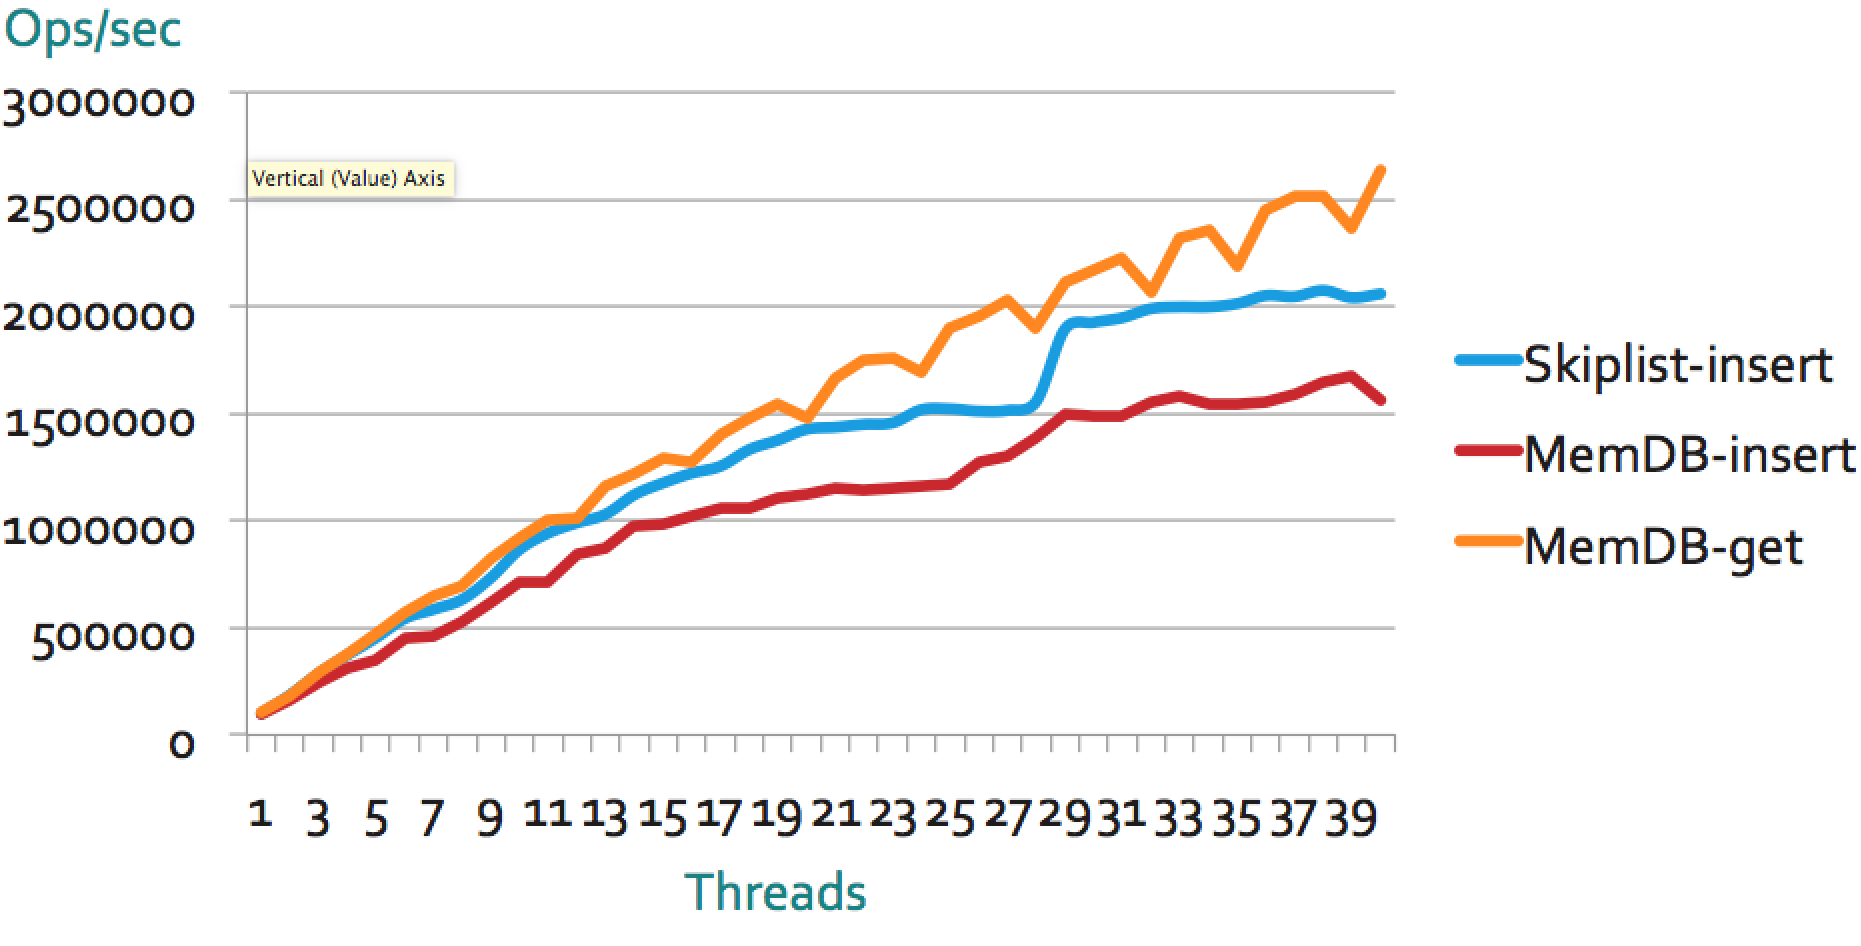
\includegraphics[scale=0.28]{images/fig-7}
\caption{Throughput with varying number of CPUs}
\label{fig:throughput-threads}
\end{figure}



\section{Future Enhancements}
The current implementation of MemDB is in golang and we have to pay for memory overheads and garbage collection cost for the entire system. The current overhead of 128B per skiplist node can be brought down to 48B per node if we rewrite the same in C. Currently, we take advantage of golang GC for safe reclamation of nodes from the Skiplist. The C implementation would require more sophisticated node garbage collector using EPOCH based collection algorithm. We are looking forward to a C implementation with superior performance soon.

    We implemented the MemDB system using skiplist as the core data structure. This helped us to build the system very quickly and the simplicity of skiplist helped us to stabilize faster. Our experiments shows that the cache unfriendliness of the skiplist keeps us away from the bonus performance boost that can be achieved by using prefetching and caching. This makes us keen to experiment with more cache friendly data structures. The MVCC layer will remain unchanged even after replacing the backbone with a non-skiplist lockfree balanced ordered search data structure.

\bibliographystyle{abbrv}
\bibliography{memdb.bib}  % vldb_sample.bib is the name of the 

\end{document}
